This section describes the experiments conducted to evaluate the proposed string and fret classifier along with the plucking position estimator. These experiments aim to demonstrate that the physical model helps to obtain a class dependent model for the classifier. They also aim to to show that it is possible to classify string and fret from the simulated feature space, and to what extent the classifier is robust towards noise. Lastly, we demonstrate an application of detailed transcription of string, fret and plucking position. The classifier is compared to~\cite{hjerrild::icassp19} and tested on 1560 recordings of two guitars from~\cite{hjerrild::icassp19}, namely an electric Les Paul Firebrand with Elixir Nanoweb (.010-.054) strings and an acoustic Martin DR with SP (.012-.052) strings. The data and MATLAB code is available online\footnote{\url{https://tinyurl.com/waspaa2019}} and we refer to the available code for implementation details. The estimation and classification is done from one short 40 ms segment for each recording, extracted at the onset event using~\cite{olivier:mirtoolbox_dafx}. %Using short segments allows for high-tempo and real-time applications.
%
\begin{figure}[t]
\centering
   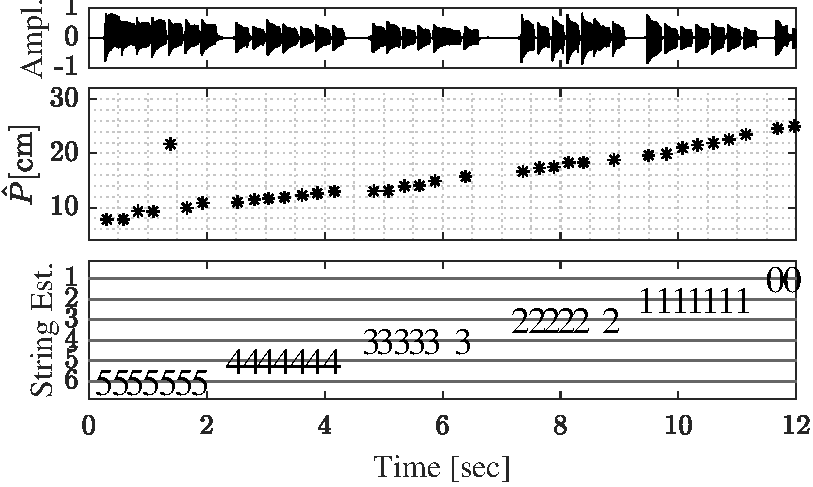
\includegraphics[width=.9\linewidth]{img/plucking_estimates}\vspace{-2mm}
   \caption{String, fret and plucking position estimates with moving plucking position and moving string and fret for electric guitar.}
   \label{fig:pluck_position_fixed_tabs} 
\end{figure}
%

Figure~\ref{fig:pluck_position_fixed_tabs} demonstrates an example application of detailed transcription, where we can observe that the proposed method is capable of estimating string, fret and plucking position, when the electric guitar is played fast with changing string and fret combinations and a moving plucking position; from the bridge towards the nut. Figure~\ref{fig:string_fret_snr} shows the sensitivity of the classifier to noise. Here, all observed signals $\vecx$ have been induced with additive white Gaussian noise (AWGN) at various levels of average signal to noise ratio (SNR) and a plausibility filter~\cite{abesser:automatic_string_detection_ml,hjerrild::icassp19} based on the equal tempered scale was applied to the classifier. The state-of-the-art model~\cite{hjerrild::icassp19} is trained on 60 recordings obtained from the 12th fret on all six strings. It can be observed that the proposed method performs slightly better than the trained model of~\cite{hjerrild::icassp19}. Interestingly, we can see from this graph that the method has a higher error-rate at a higher SNR for the electric guitar than for the acoustic, which implies that the higher harmonics of the acoustic has a relatively higher amount of energy than in the electric signal, which can be related to the electronics of the transducers on these guitars. 

Finally, we can evaluate the detailed and class dependent simulation of the feature space and compare it to estimates obtained with~\cite{hjerrild::icassp19}. In this simulation, all string properties are normally distributed with a standard deviation specified as 0.5\% of their respective mean value (see the available evaluation code). The resulting distributions are shown in Figure~\ref{fig:string_and_fret_model}, where the consistency between simulation and measurement can clearly be observed. Note here, that the simulation has a detailed and class dependent distribution of $\omega_0$ and $B$, which is not possible to obtain with state-of-the-art method~\cite{hjerrild::icassp19}. We also emphasize that computational time for a simulating a model with 500 realizations of 78 classes takes 45 ms on an i7 processor using MATLAB. %The class dependency of the simulation could be the reason why the simulated model performs slightly better than~\cite{hjerrild::icassp19} in Figure~\ref{fig:string_fret_snr}.
%
\begin{figure}[t]
\centering
   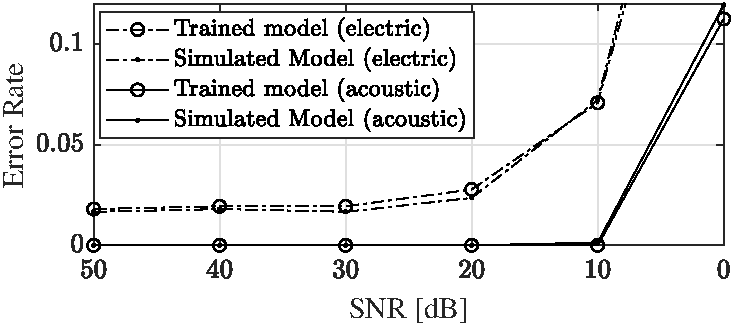
\includegraphics[width=.85\linewidth]{img/SNRfig_both.pdf}\vspace{-2mm}
   \caption{String, fret classification error rate as a function of SNR. Each marker represents 720 classifications. The trained model represents~\cite{hjerrild::icassp19} and the simulated model is the proposed method.}
   \label{fig:string_fret_snr} 
\end{figure}
%
\begin{figure}[t]
\centering
   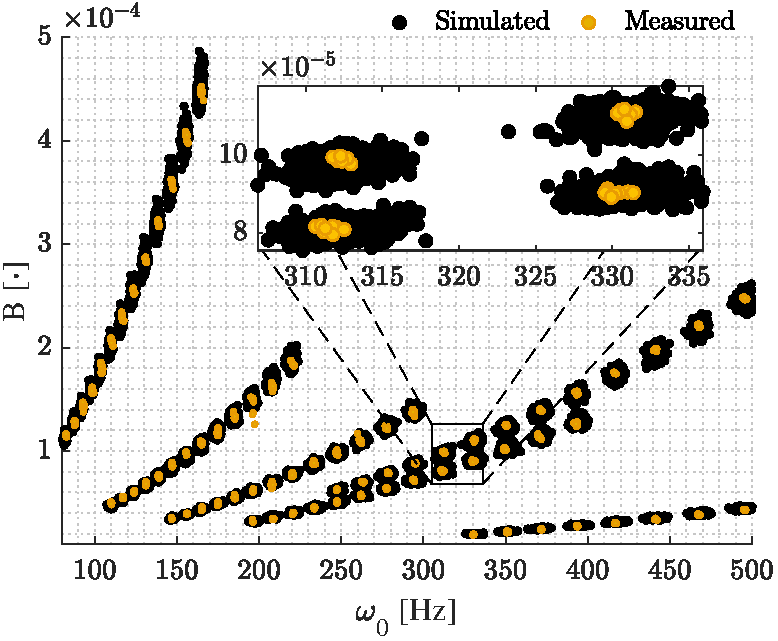
\includegraphics[width=.85\linewidth]{img/w0_vs_B3.pdf}\vspace{-2mm}
   \caption{Comparison of simulated random variables to the measured estimates of the features for the acoustic guitar. For each class there is 500 simulated values and 10 estimated measurements.}
   \label{fig:string_and_fret_model} 
\end{figure}
%